% -*- mode: LaTeX; coding: utf-8 -*-
% Typeset with: XeLaTeX

\documentclass{beamer}
\mode<presentation>
{
  \usetheme[progressbar=foot,numbering=fraction,background=light,block=fill]{metropolis} 
  \usecolortheme{default} % or try albatross, beaver, crane, ...
  \usefonttheme{default}  % or try serif, structurebold, ...
  \setbeamertemplate{navigation symbols}{}
  \setbeamertemplate{caption}[numbered]
  %\setbeamertemplate{frame footer}{My custom footer}
}
\centering

% Commands for tansparent block and to correct the small line space with the title.
% \metroset{block=transparent}
% \vspace{0pt}

\usepackage{graphicx,pgfplots,tikz,tikz-3dplot}
\graphicspath{ {./figures/} }
\usepackage{hyperref,xcolor}
\newcommand{\link}[2]{\href{#1}{\textcolor{blue}{\underline{#2}}}}

% Main document
\begin{document}
\title{Road segmentation and alignment}
\subtitle{Geometric Data Analysis}
\author{Thomas Pappas\\ \link{mailto:thpappas@di.uoa.gr}{thpappas@di.uoa.gr}}
\date{November 26, 2020}
\maketitle

\begin{frame}{Agenda}
  \tableofcontents[hideallsubsections]
\end{frame}

\section{Road segmentation}

\subsection{Introduction}

\begin{frame}{Road segmentation}
  \begin{block}{What is Road segmentation?}
    Partitioning of roads into segments in order to represent and compare map information in a more meaningful and easier to analyse way\\
    (various applications e.g. traffic analysis, anomaly detection)
    \begin{itemize}
      \item A segment consists of two or more nodes
      \item Line segment is a segment consisting of two nodes
    \end{itemize}
  \end{block}
  
  \begin{block}{Types of road segmentation}
    \begin{itemize}
      \item Segmentation by junction
      \item Segmentation by curvature
    \end{itemize}
  \end{block}
\end{frame}

\begin{frame}{Road segmentation}
  \begin{block}{Highways}
    \begin{itemize}
      \item High-performance roads
        \begin{itemize}
          \item Motorway
          \item Trunk
          \item Primary
          \item Secondary
          \item Tertiary
        \end{itemize}
      \item Low-performance roads
        \begin{itemize}
          \item Residential
          \item Unclassified
          \item Service
        \end{itemize}
      \item Link roads
    \end{itemize}
  \end{block}
\end{frame}

\subsection{Segmentation by curvature}

\begin{frame}{Segmentation by curvature}
  \begin{block}{Curve radius}
    Every set of three points defines a triangle. We call curve radius the radius of the triange's circumcircle.
  \end{block}

  \begin{block}{Curvature}
    The curvature of a line segment is the mean of the curve radius of the sets its two points participate. (Figure 1)
  \end{block}

  \begin{block}{When to create a segment?}
    We keep the minumum curvature of the segment under construction. We create a new segment when we occur a line segment with a curvature with high augmentation compared to the min curvature.
  \end{block}
\end{frame}

\begin{frame}{Curvature}
  \begin{figure}[h]
    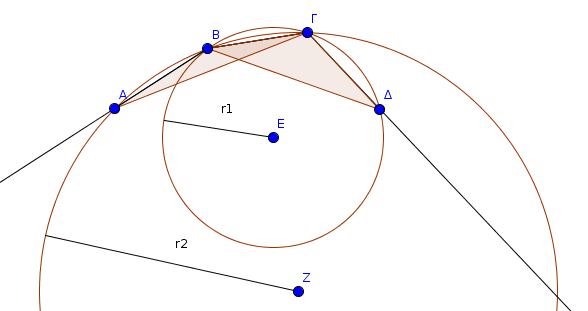
\includegraphics[width=0.8\textwidth]{line_segment_curvature}
    \caption{The curvature of the line segment $B\Gamma$ is $(r_1+r_2)/2$.}
  \end{figure}
\end{frame}

\begin{frame}{Formula for regulated segmentation}
  \metroset{block=transparent}
  \begin{block}{}
    If we define
    \begin{itemize}
      \item $P$ the set of points in the highway
      \item $H$ the set of points in the highway that have been divided to segments
      \item $\rho$ a minor positive number (e.g. $\rho = 8$)
      \item $\lambda$ the length of the under construction segment
      \item $\mu$ the mean length of all the highways of the same category
    \end{itemize}
    then when
    \[
      |P| > (|H|/(|H|/\rho + 1)) \textrm{ and } (\lambda > \mu)
    \]
    are both true, create a new segment.\\
    Note: Invented through experimental processes.
  \end{block}
\end{frame}


\begin{frame}{Segmentation by curvature}
  \begin{block}{Algorithm}
    Input: A set of points $P$\\
    Output: A set of segments (set of points from $P$)
    \begin{enumerate}
      \item If $|P| < 3$, create a single segment and exit
      \item Initialise min-curvature to $0$
      \item Iterate through the line segments
        \begin{enumerate}
          \item If first segment, initialise a segment, set min-curvature equal to the current one and continue
          \item If last segment, add the last point to the segment and finalise it
          \item If the curvature has high augmentation compared to the min-curvature, finalise the segment under construction and intiate a new one with the current line segment;\\
          set min-curvature as the current one
          \item Else add the second point to the segment, update min-curvature (if needed) and continue
        \end{enumerate}
    \end{enumerate}
  \end{block}
%  \begin{block}{Complexity}
%    $\mathcal{O}(n)$
%  \end{block}
\end{frame}

\begin{frame}{Segmentation by curvature - Example}
  Curvature segment criteria: $|currentCurve - minCurve| > minCurve$
  \begin{scriptsize}
    \begin{table}
      \caption{Segmentation by curvature, New York (Brooklyn)}
      \label{table:1}
      \begin{tabular}{ l | c c c c }
        \hline
        Highway type & \# & \#segments & \#segments (with formula) & mean length\\
        \hline
        Unclassified & $5$ & $10$ & $11$ & $108.17$\\
        Primary link & $6$ & $6$ & $6$ & $67.64$\\
        Tertiary & $45$ & $79$ & $83$ & $411.60$\\
        Motorway link & $20$ & $26$ & $27$ & $128.99$\\
        Motorway & $7$ & $15$ & $17$ & $663.07$\\
        Secondary & $275$ & $344$ & $348$ & $139.34$\\
        Residential & $756$ & $1069$ & $1109$ & $331.72$\\
        Service & $108$ & $219$ & $227$ & $146.47$\\
        Unused & $543$ & $1158$ & $1204$ & $112.82$\\
        Secondary link & $2$ & $2$ & $2$ & $27.81$\\
        Primary & $240$ & $285$ & $286$ & $110.53$
      \end{tabular}
    \end{table}
  \end{scriptsize}
\end{frame}

\section{Road alignment with Descrete Fréchet Distance}

\begin{frame}{Descrete Fréchet Distance (DFD)}
  Distance measure for matching two geometric objects in $2D$ or $3D$.
  \begin{block}{For reference}
    For two polygonal curves $P$ and $Q$ and the set of all possible travesals $T$
    \[
      d_F(P,Q) = \min_T \max_{(i_k,j_k) \in T} d(p_{i_k}, q_{j_k})
    \]
    Computed using dynamic programming.
  \end{block}
\end{frame}

\subsection{Calculating DFD with translation and rotation}

\begin{frame}{Calculating DFD with translation and rotation $2D$}
  \begin{block}{Problem}
    For  two polygonal curves $P$ and $Q$ find the minimum DFD value for all possible translations and rotations.
  \end{block}
  
%  \begin{block}{Solution for 2D}
%    Long story
%  \end{block}
  
  \begin{block}{Theorem 2\footnotemark}
    For minimizing the discrete Fréchet distance between two $2D$ polyg-onal chains under translation and rotation, we have an $\mathcal{O}(m^4n^4\log{}(1/\epsilon))$ time $1+\epsilon$ approximation algorithm and an $\mathcal{O}(m^4n^4\log{}(m+n))$ time exact algorithm.
  \end{block}
  \footnotetext[1]{Jiang M, Xu Y, Zhu B. Protein structure-structure alignment with discrete Fréchet distance. J Bioinform Comput Biol. 2008 Feb;6(1):51-64. doi: 10.1142/s0219720008003278. PMID: 18324745.}
\end{frame}

\begin{frame}{Calculating DFD with translation and rotation $2D$}
  \begin{block}{The idea behind Theorem 2}
    \begin{itemize}
      \item Runtime to check the DFD for an arbitrary translation: $\mathcal{O}(mn)$
      \item Solve the decision problem for $\epsilon > 0$
        \begin{itemize}
          \item Check transformations for every $4$ (at most) vertices
          \item i.e. hold $3$ vertices of reference, so runtime becomes $\mathcal{O}((mn)m^3n^4) = \mathcal{O}(m^4n^4)$
        \end{itemize}
      \item Either use binary search to approximate the min DFD\\
        $1+\epsilon$ approximation algorithm
      \item Or use Cole’s sorting trick\footnotemark$^,$\footnotemark\\
        $\mathcal{O}(m^4n^4\log{}(m+n))$ time exact algorithm
    \end{itemize}
    \footnotetext[2]{Alt H, Knauer C, Wenk C, Matching polygonal curves with respect to the Fréchet
distance, in Proceedings of the 18th Annual Symposium on Theoretical Aspects of
Computer Science (STACS’01), pp. 63–74, 2001.}
    \footnotetext[3]{Cole R, Slowing down sorting networks to obtain faster sorting algorithms, J ACM 34:200–208, 1987.}
  \end{block}
\end{frame}

\begin{frame}{Calculating DFD with translation and rotation $3D$}
  \begin{block}{Algorithm for $3D$}
    If we apply the same idea for $3D$ then we need $6$ vertices of reference and we therefore get an algorithm of complexity $\mathcal{O}((mn)^7)$ (ignoring the log factors) for transformations under translation and rotation.\\
    We will instead present a faster intuitive heuristic.
  \end{block}
\end{frame}

\begin{frame}{Calculating DFD with translation and rotation $3D$}
  \begin{block}{Observations}
    \begin{itemize}
      \item Given $3D$ chain $C$ of $n$ vertices, each vertex $c_i$ is a $3D$ vector $\vec{c_i}$
      \item The center $c$ is the vector $\vec{c} = \frac{\sum_i \vec{c_i}}{n}$
    \end{itemize}
    For two polygonal chains $A,B$ where\\
    $A = \langle \alpha_1,\alpha_2,\cdots,\alpha_m \rangle$ and $B = \langle b_1,b_2,\cdots,b_n \rangle$
    \begin{itemize}
      \item if $d_F(A,B) = \epsilon$ then $d(\alpha_1,b_1) \leq \epsilon$ and $d(\alpha_m,b_n) \leq \epsilon$
      \item If $\epsilon < \frac{1}{2}\min_{i < m} |\alpha_{i+1}-\alpha_i|$ or $\epsilon < \frac{1}{2}\min_{i < n} |b_{i+1}-b_i|$, then the Fréchet alignment of $A$ and $B$ must contain only $1-1$ matches, i.e $m = n$ and for $0 \leq i \leq n$ we have $d(\alpha_i,b_i) \leq \epsilon$.\\
      Therefore for $\alpha,b$ the centers of $A,B$ respectively, $d(\alpha, b) \leq \epsilon$
    \end{itemize}
  \end{block}
\end{frame}

\begin{frame}{Calculating DFD with translation and rotation $3D$}
  \begin{block}{Heuristic for $3D$}
    From the above observations, we see we can use the three points (endvertices and center) as reference points.
    \begin{enumerate}
      \item Translate $B$ such that the centers $\alpha$ and $b$ coincide
      \item Rotate $B$ around $b$ such that $\vartriangle \alpha\alpha_1\alpha_m$ and $\vartriangle bb_1b_n$ are coplanar
        \begin{itemize}
          \item Also such that $\frac{\vec{\alpha_1}+\vec{\alpha_m}}{2}-\vec{\alpha}$ and $\frac{\vec{b_1}+\vec{b_n}}{2}-\vec{b}$ have the same direction
        \end{itemize}
      \item Randomly select two vertices from $B$. Rotate $B$ for a small angle around the axis through the two vertices; if DFD does not decrease, rotate back
      \item Repeat step $3$ (tuning) for a number of times
    \end{enumerate}
  \end{block}
\end{frame}

\begin{frame}{Examples}
  \begin{small}
    \begin{table}
      \caption{DFD comparison of two highways from each category with the highest same size. We compute the DFD under translation $d_F$ (tr), DFD under translation and rotation $\min d_F$ and the c-RMSD.}
      \label{table:2}
      \begin{tabular}{ l | c c c c c }
        Highway type & $|A|$ & $|B|$ & $d_F (tr)$ & $\min d_F$ & c-RMSD\\
        \hline
        Unclassified & $10$ & $10$ & $129.05$ & $60.61$ & $40.45$\\
        Primary link & $2$ & $2$ & $67.05$ & $54.37$ & $54.37$\\
        Tertiary & $11$ & $11$ & $210.24$ & $63.06$ & $53.77$\\
        Motorway link & $5$ & $5$ & $24.83$ & $21.28$ & $17.52$\\
        Motorway & $9$ & $9$ & $168.15$ & $90.05$ & $53.28$\\
        Secondary & $14$ & $14$ & $205.50$ & $177.13$ & $81.54$\\
        Residential & $27$ & $27$ & $887.77$ & $645.15$ & $366.53$\\
        Service & $28$ & $28$ & $171.24$ & $56.25$ & $41.71$\\
        Unused & $37$ & $37$ & $186.84$ & $133.62$ & $59.36$\\
        Secondary link & $3$ & $3$ & $23.95$ & $6.87$ & $5.90$\\
        Primary & $11$ & $11$ & $415.89$ & $199.93$ & $129.75$\\
      \end{tabular}
    \end{table}
  \end{small}
\end{frame}

\begin{frame}{Examples}
  \begin{block}{Some conclusions}
    \begin{itemize}
      \item Translation only DFD can be a lot larger than if we also allow rotation
      \item c-RMSD seems to have better results for alligning the two lines
    \end{itemize}
  \end{block}
\end{frame}

%\begin{frame}{Examples}
%  \begin{figure}
%    \begin{tikzpicture}
%    \begin{axis}
%    [   view={-45}{60},
%      xmin=0,xmax=5,
%      ymin=0,ymax=5,
%      zmin=0, zmax=5,
%    ]
%    \addplot3[
%      surf,color=red
%    ] 
%    coordinates {
%      (0,0,0) (0,1,0) (0,2,0)
%      (1,0,0) (1,1,0.6) (1,2,0.7)
%      (2,0,0) (2,1,0.7) (2,2,1.8)
%    };
%    \end{axis}
%
%    \end{tikzpicture}
%  \end{figure}
%\end{frame}

%\section{Bibliography}

\begin{frame}{Bibliography}
  \begin{itemize}
    \item Dimitrios - Nikolaos Konstantakis, Geometrical Road Segmentation and Clustering, BSc Thesis, National and Kapodistrian University of Athens, Department of Informatics and Telecommunications, 2018 April
    \item Jiang M, Xu Y, Zhu B. Protein structure-structure alignment with discrete Fréchet distance. J Bioinform Comput Biol. 2008 Feb;6(1):51-64. doi: 10.1142/s0219720008003278. PMID: 18324745.
  \end{itemize}
\end{frame}

\end{document}
